\section{Pályakövetési feladatok}

A robot pályakövetési feladatát megfogalmazhatjuk úgy, hogy tudjunk eljutni A pontból B pontba, ha ismerjük a robot síkbeli pozícióját és az orientációját egy térképen, amely megfelel a környezetnek, látható az \ref{fig:PositionController} ábrán.
A \ref{fig:PositionController} ábrán látható, hogy felveszünk egy pozitív és egy negatív irányt a szögre nézve, az orientációkat mindig [0\degree 360\degree] között kell megadjuk. A robotnak mindig arra kell fordulnia, amerre a szög a legkisebb, azért, hogy minél kevesebbet keljen mozogjon.
A kiinduló állapotban a robot kezdetben az A pontban van és az orientációja $\beta_0$ és a B pontba szeretnénk eljutni egyenes vonalban. Így a robotnak kezdetben a célra kell fordulnia és ezután haladhat előre, miközben korrigálja az orientációs hibákat.
Első lépésben a robotnak fordulnia kell $error$ szöget, hogy $\beta_1$ irányba mutasson és ezután haladhat a cél fele.


\begin{figure}[H]
    		%trim = bal also jobb felso
   \fbox{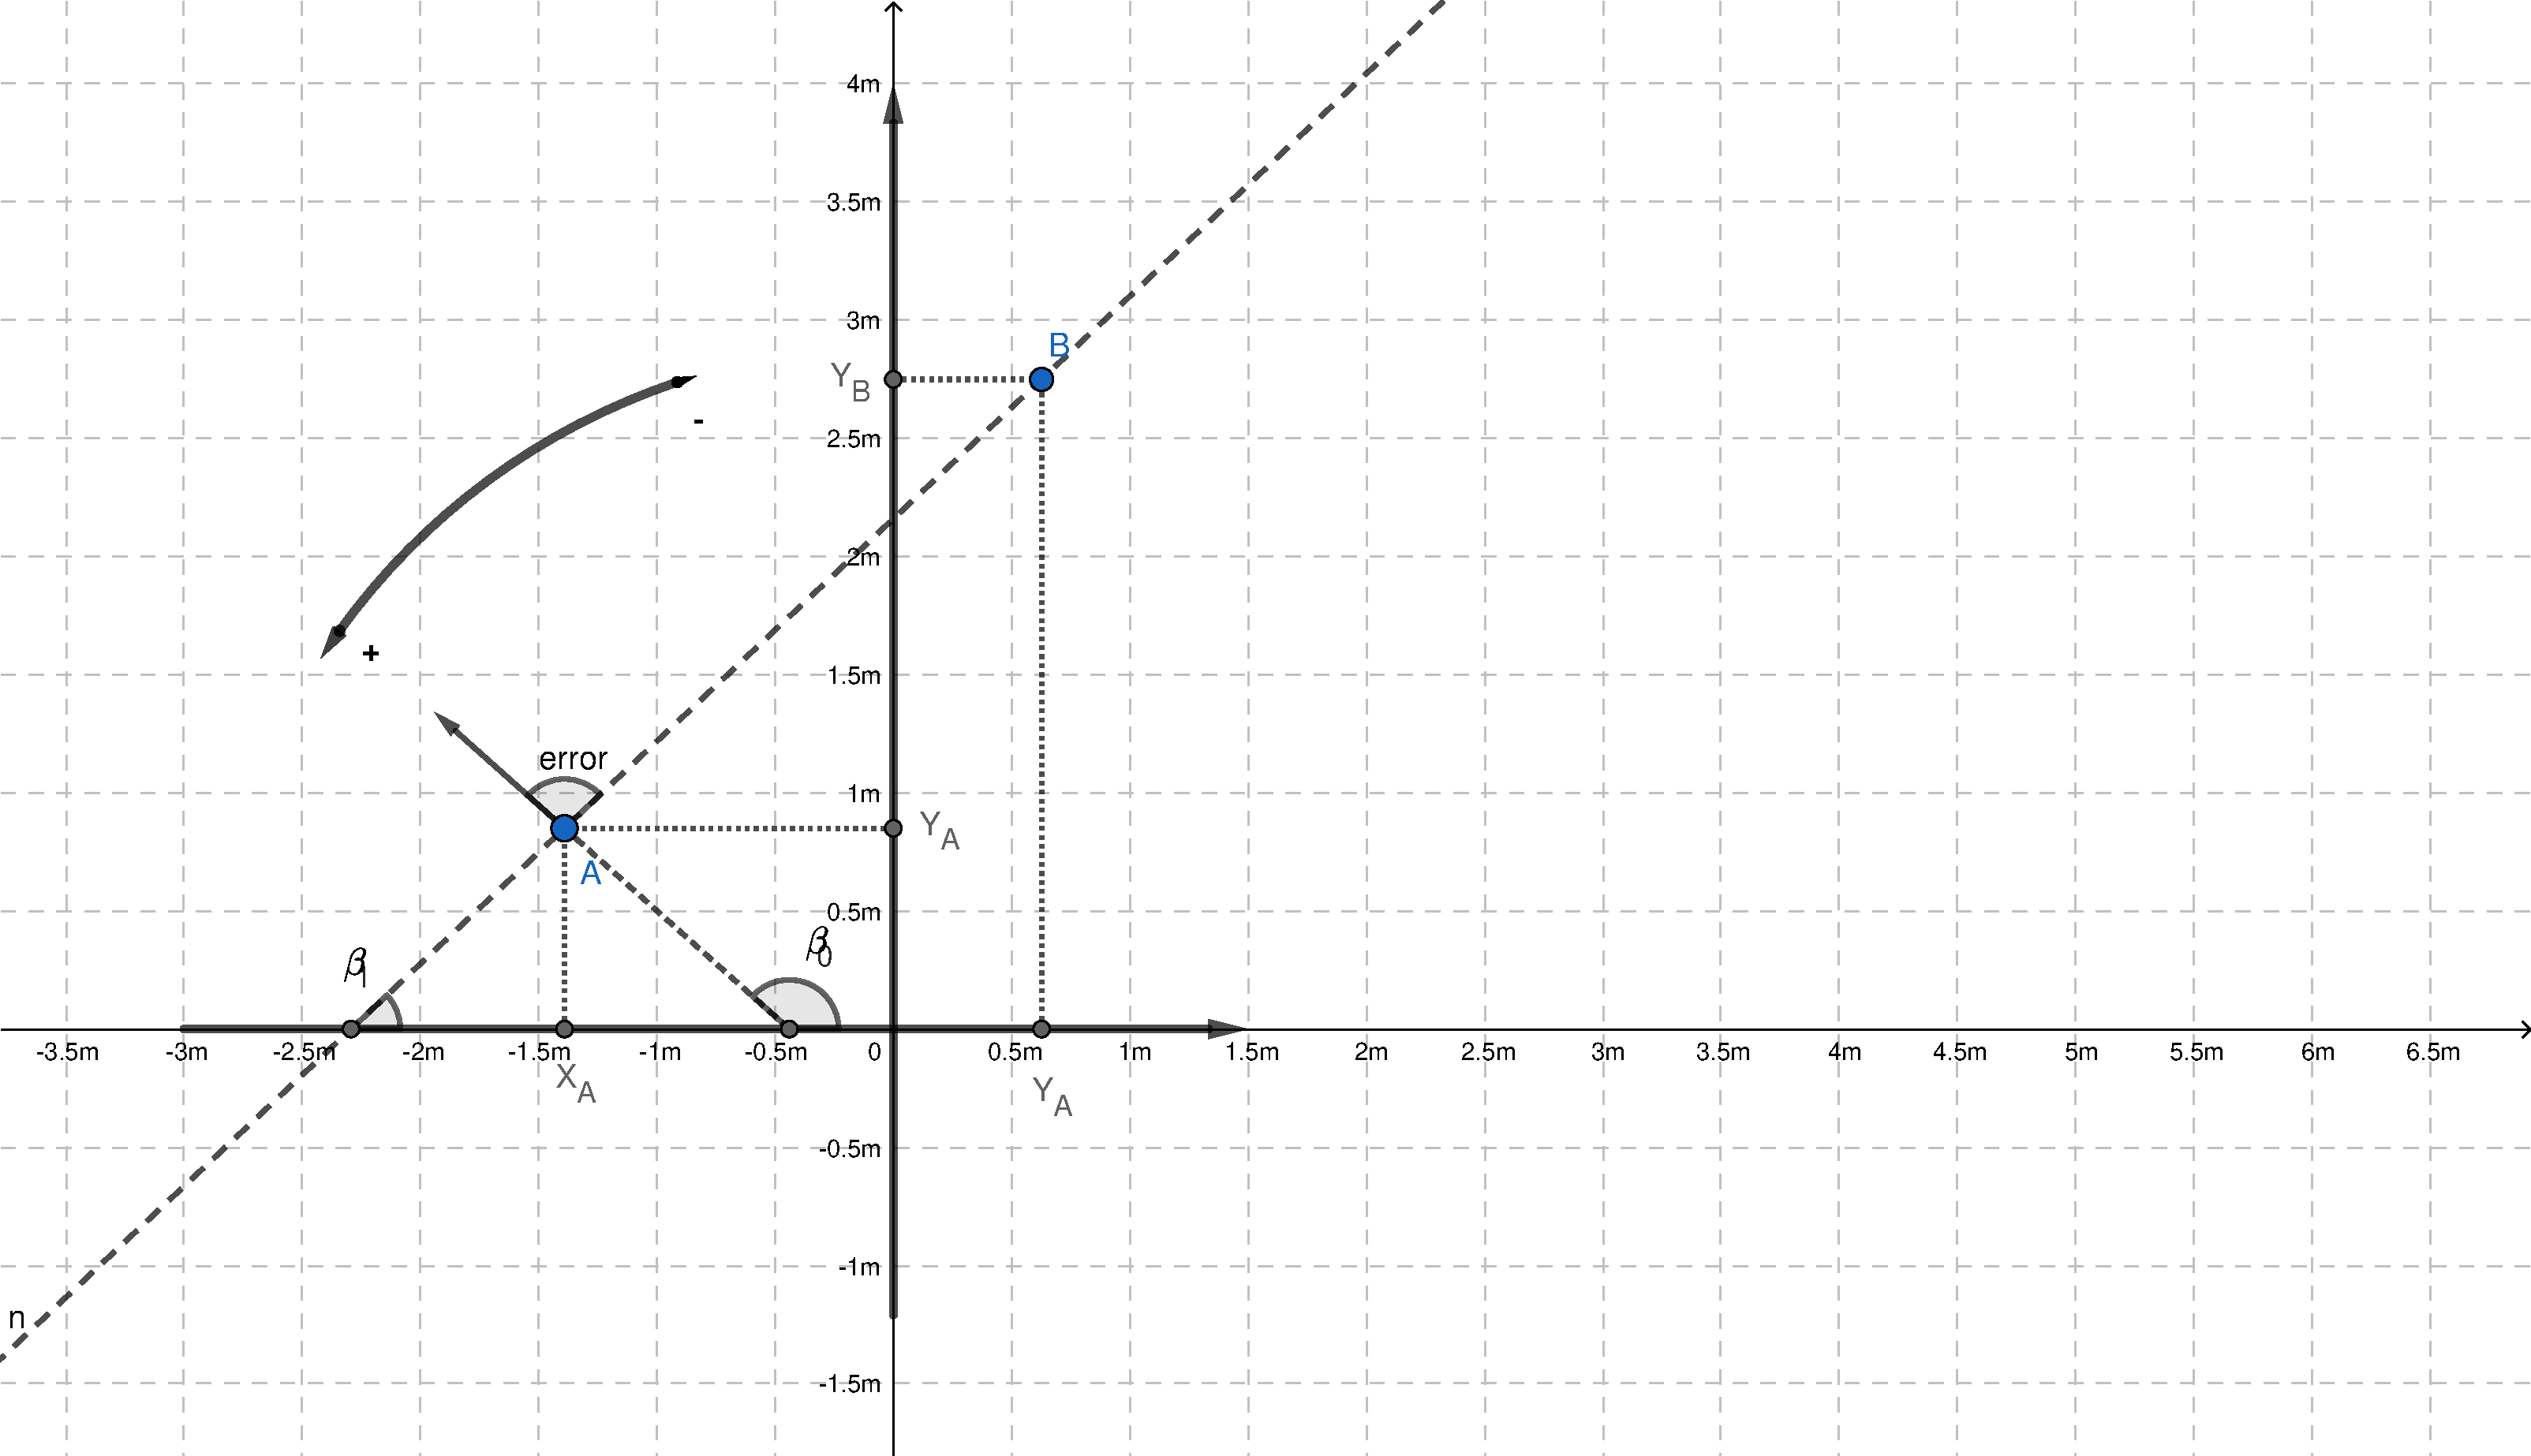
\includegraphics[width=1\columnwidth,trim=3cm 6cm 27cm 2cm,clip]{tikz/PositionController.pdf}}
  \caption{Robot pozíció szabályzása}
  \label{fig:PositionController}
\end{figure}


A pályakövetési algoritmus látható alább. Az  előírt irányt $tan^{-1}$ függvény segítségével határozzuk meg, ismerve X és Y tengelyen a hibák nagyságát. A Rotate($e_\alpha$,$\Omega_{max}$) függvényben alkalmazunk egy PI típusú szabályzót, melynek a feladata a szöghiba 0-hoz való közelítése. A Vx(d,$V_max$) a robot lineáris sebességének a szabályzását látja el egy PI típusú szabályzó, célja a robot és a kitűzött cél távolságának a csökkentése. 
A távolságszabályzó bemenetét súlyozzuk $1/e_\alpha$ értékkel, hogy ameddig nincs a robot irányban, addig ne domináljon távolságszabályzó.

\begin{algorithm}
   \caption{Pályakövetés Algoritmusa}
    \begin{algorithmic}[1]
     %\Function{GetNextControl}{$X_a,Y_a\alpha$}
      \Function{GetNextControl}{$X_a,Y_a,\alpha_a,X_t,Y_t,\alpha_t,Tr,Tr_\alpha,\Omega_{max},V_{max}$}
      %\Comment{Ahol X,Y - pozicio a térképén, \alpha irány, a - aktuális, t - előírt, Tr - pozicio hiba küszöb, $Tr_{\alpha}$ - szöghiba küszöb,${\Omega}_{max}$ maximális forgási sebesseg, $V_{max}$ maximális haladási sebesség. }
      
       \State $e_x = X_a-X_t$
       \State $e_y = Y_a-Y_t$
       \State $d=\sqrt{e_x^2+e_y^2}$
       \State $\alpha_i=dir(X_a,Y_a,X_t,Y_t)$ \Comment{Két ponton átmenő egyenes iránytényezője}
       \State $e_\alpha=\alpha_i-\alpha_a$
            \If {$e_\alpha > Tr_\alpha$} \Comment{Fordulj a cél fele}
                \State $\Omega = Rotate(e_\alpha,\Omega_{max}) $
                \State $V_x = 0 $
            \Else \Comment{Haladj a cél fele és korrigáld az elfordulást}
                
                \State $\Omega = Rotate(e_\alpha,\Omega_{max}) $
                \State $V_x = Vx(d*1/e_\alpha,V_{max})$
            \EndIf
     
            \If {$e_\alpha < Tr_\alpha$ és $d<Tr$} \Comment{Kívánt pozícióban}
                \State $\Omega = 0$
                \State $V_x = 0 $
            \EndIf
        
       \EndFunction

\end{algorithmic}
\end{algorithm}



Az algoritmus tesztelésére MATLAB/Simulink környezetet használtam. A robot kinematikai modellt az \ref{eq:allapot} egyenlet alapján modelleztem, a pozíciók (X,Y) és az irány meghatározására integráltam a lineáris és szögsebességeket. 

A \ref{fig:SimPoseCont} ábrán láthatjuk a szimulációs eredményeket, amint a robot egy végtelen jelhez hasonló pályát követ.

\begin{figure}[H]
	\setlength{\fboxsep}{0pt}
	\setlength{\fboxrule}{0pt}
	
    \begin{center}  	
    		%trim = bal also jobb felso
    	\fbox{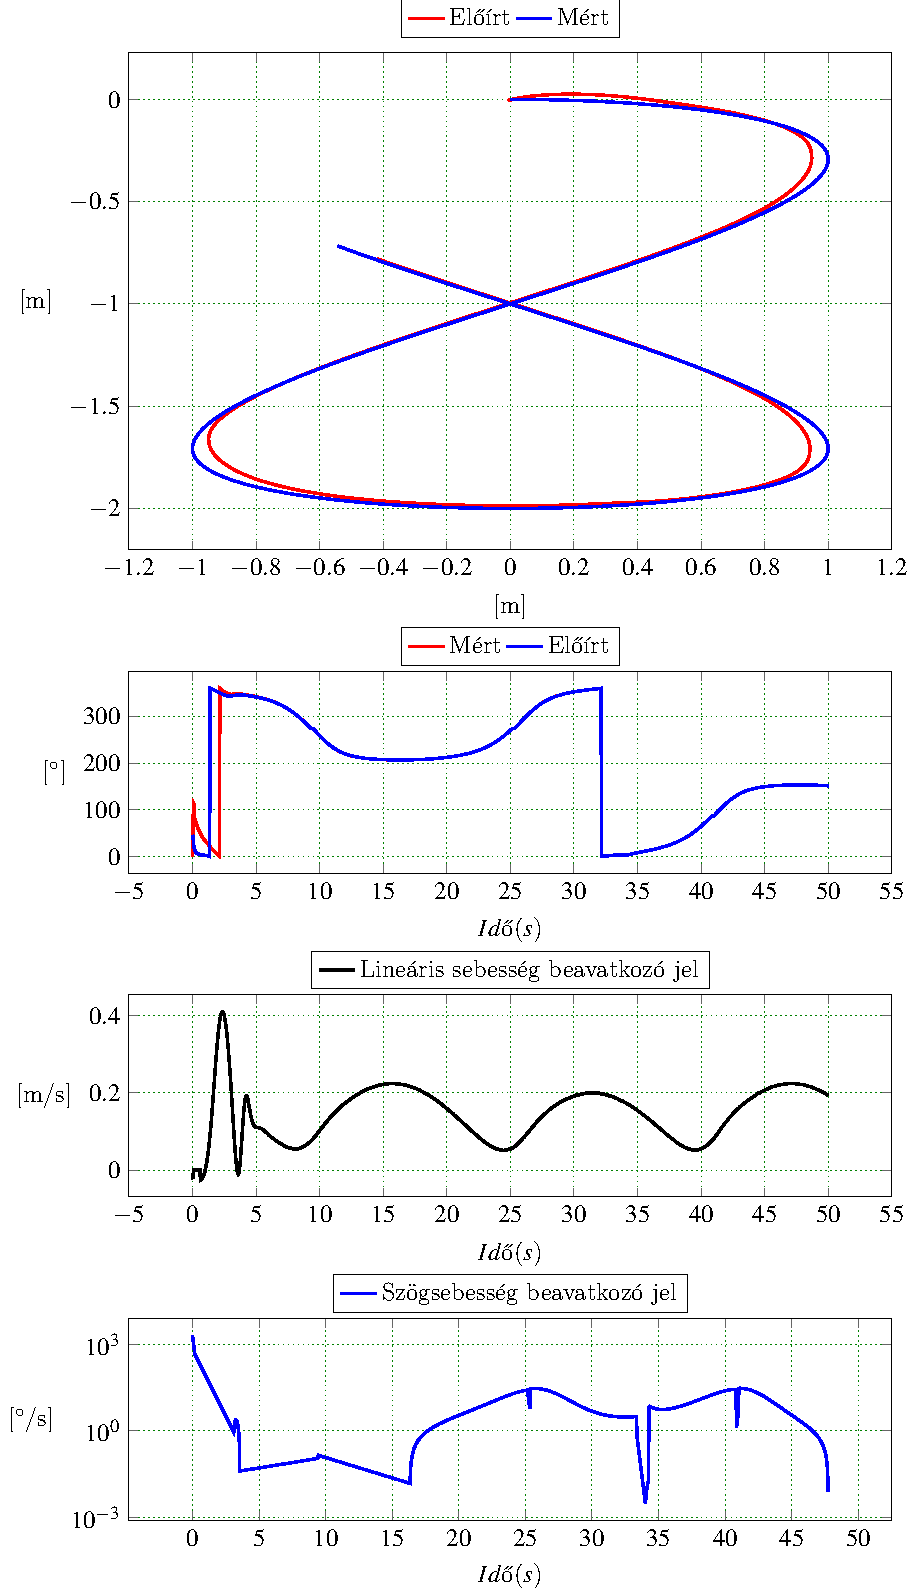
\includegraphics[width=0.9\columnwidth,trim=0cm 0cm 0cm 0cm,clip]{tikz/SimPoseCont.pdf}}
    \end{center}  
    
  	\caption{Robot pozíció szabályzása}
  	\label{fig:SimPoseCont}
\end{figure}
